\documentclass{article}
\usepackage[utf8]{inputenc}
\usepackage{amsmath}
\usepackage{graphicx}
\usepackage{float}

\title{Exam questions}
\author{Cristian Manuel Abrante Dorta}
\date{April 2020}

\begin{document}

\maketitle

\section{Define the idempotence property that is satisfied by certain operators.}

Idempotence is a property that many operators in mathematics and computer science hold. Informally, we can say that an operator is idempotent if the result of the application of it several times does not differ from the application of it only one time.\\

Formally, we can say that certain operator ($\varphi$) is idempotent if it satisfies the following property:

\begin{equation}
    \varphi(I) = \varphi(\varphi(I)) = \varphi(\varphi(\cdots \varphi(I))
\end{equation}

There are many examples of idempotent operators. In a daily life example, an idempotent operation could be washing our hands; the result of washing our hands is equal if we apply the operation once or if we apply it many times.\\

In the field of image processing, we can affirm that the opening is an idempotent function. We can observe an example of an image whose application of the erosion gives the same result even if it is applied twice.

\begin{figure}[!h]
\minipage{0.32\textwidth}
  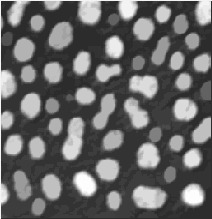
\includegraphics[width=\linewidth]{report/exam/images/immed_gray_inv_20051218_frgr4.jpg}
  \caption{Original image without operations}\label{fig:image-1}
\endminipage\hfill
\minipage{0.32\textwidth}
  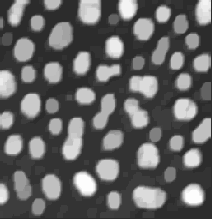
\includegraphics[width=\linewidth]{report/exam/images/exercise_05a_output-01_1.png}
  \caption{Image after applying opening once}\label{fig:awesome_image2}
\endminipage\hfill
\minipage{0.32\textwidth}%
  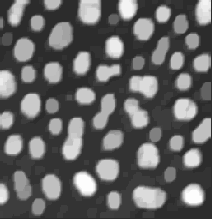
\includegraphics[width=\linewidth]{report/exam/images/exercise_05a_output-02.png}
  \caption{Image after applying opening twice}\label{fig:awesome_image3}
\endminipage
\end{figure}

\section{True or false questions.}

\begin{itemize}
    \item Indicate whether dilations ($\delta$) and erosions ($\epsilon$) are idempotent. (\textbf{FALSE})
    \item Indicate whether openings ($\gamma$) and closings ($\varphi$) are idempotent. (\textbf{TRUE}).
    \item Indicate whether alternated filters ($\varphi\gamma$ and $\gamma\varphi$) are idempotent. (\textbf{TRUE})
\end{itemize}

\section{Enumerate one segmentation algorithm based in neighbourhood processing.}

One example of an algorithm which uses neighbourhood processing for obtaining the different segments of an image is the \textbf{grassfire algorithm}. \\

This algorithm visits all the pixels of the image in order to evaluate the region that this pixel belongs to. For this evaluation, it defines a neighbourhood of pixels with a certain connectivity (4-connectivity or 8-connectivity), each pixel of this neighbourhood that have the same gray level of the central pixel will be added to a queue and explored in a consecutive way, until this queue is empty and all the pixels of images have been assigned.

\begin{figure}[H]
    \centering
    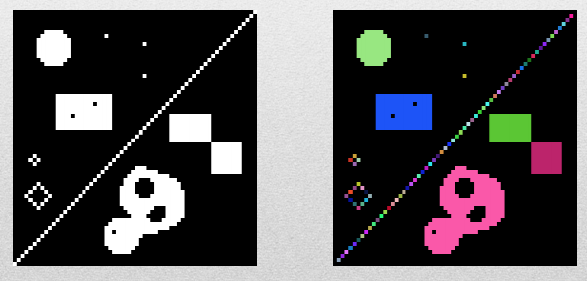
\includegraphics[scale=0.35]{report/exam/images/grassfire.png}
    \caption{Example of the output of the grassfire procedure}
    \label{fig:my_label}
\end{figure}

\section{Which kind of algorithms / techniques are commonly used for semantic image segmentation?}

Semantic image segmentation is the field of image processing that studies the techniques used for detecting the different regions or segments which are present in an image, and at the same time gives a semantic meaning for those regions, in a similar way than a human would do it.\\

All the \textit{state of the art} techniques used for semantic image segmentation are based on deep learning algorithms. Deep learning is a subfield of artificial intelligence and machine learning which uses the concept of deep neural networks, networks with two or more hidden layers. Those networks have the capacity of discovering and extrapolate complex patterns in data, or images, when applied to our field of study. \\

One type of deep neural networks which are suitable for image processing are \textbf{convolutional neural networks} (CNN), those networks apply the mathematical operation of convolution in order to learn the complex patterns of images in the successive layers that it has. \\

For addressing the semantic segmentation problem, There are mainly three approaches:

\begin{itemize}
    \item \textbf{Naive approach (sliding window)}: This first approach is based on a sliding window that will explore all the different pixels of the image, and use the region of the pixel with a classification network in order to assign a label to it. The main drawback of this method is that it is computationally inefficient.
    \begin{figure}[H]
        \centering
        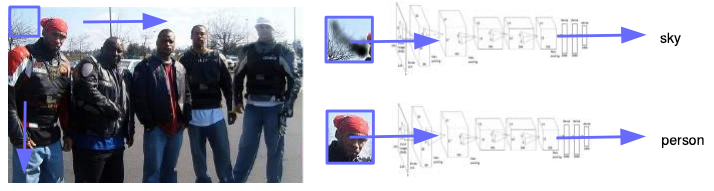
\includegraphics[scale=0.4]{report/exam/images/sliding-window.png}
        \caption{Sliding window example}
        \label{fig:my_label}
    \end{figure}
    
    \item \textbf{Two stage approaches}: In those algorithms we have two CNNs, the first one is used for detecting which are the segments (usually bounding boxes) present in the image, and the second neural network is used for classifying those regions in one of the expected classes.
    \begin{figure}[H]
        \centering
        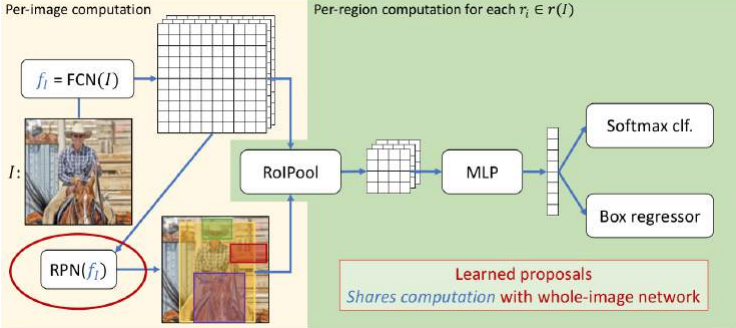
\includegraphics[scale=0.3]{report/exam/images/two-stage.png}
        \caption{Two stage scheme}
        \label{fig:my_label}
    \end{figure}
    
    Examples of those algorithms are: R-CNN \cite{rcnn}, Fast RCNN \cite{fastrcnn} or Faster RCNN \cite{fasterrcnn}
    
    \item \textbf{One stage approach}: In this approach, we only have one neural network which processes the image and then calculates the bounding boxes and the classes. The main drawback of this method is that the complexity of the network increases in a significant way, but it reduces the computation time, being a good solution for real-time image processing.\\
    
    \begin{figure}[H]
        \centering
        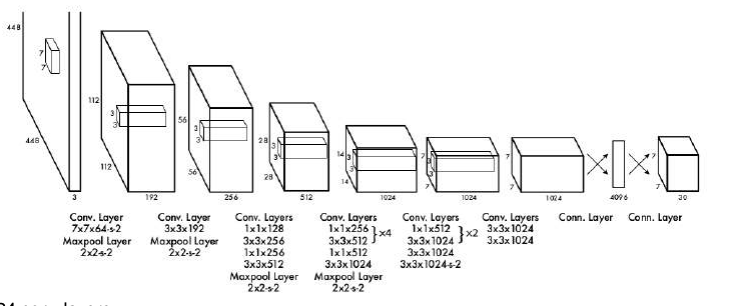
\includegraphics[scale=0.3]{report/exam/images/yolo.png}
        \caption{Architecture of YOLO network}
        \label{fig:my_label}
    \end{figure}
    
    The state of the art of this type of algorithms is \textbf{YOLO} (You only look once)\cite{yolo}
\end{itemize}

%%%%%%%%%%%%%%%%%%%%%%%%%%%%%%%%%%%%%%%%%
\begin{thebibliography}{9}
\bibitem{rcnn}
   Girshick, Ross and Donahue, Jeff and Darrell, Trevor and Malik, Jitendra
    \newblock {\em Rich feature hierarchies for accurate object detection and semantic segmentation}, 2014.

\bibitem{fastrcnn}
    Girshick, Ross
    \newblock{\em Fast r-cnn}, 2015
    
\bibitem{fasterrcnn}
    Ren, Shaoqing and He, Kaiming and Girshick, Ross and Sun, Jian
    \newblock{\em Faster r-cnn: Towards real-time object detection with region proposal networks}, 2015

\bibitem{yolo}
    Redmon, Joseph and Divvala, Santosh and Girshick, Ross and Farhadi, Ali
    \newblock{\em You only look once: Unified, real-time object detection}, 2016

\end{thebibliography}

\end{document}
